\section{Experimentos e resultados} 

Para poder fazer cada experimento foi utilizado o programa toysat \cite{ToySAT14} e um script para ter varios threads em paralelo tão para gerar os datos como para executar toysat solver. Além, os tempos mostrados nos gráficos são os tempos promedios de execução para cada configuração de parâmetros.

\subsection{Experimento 1}
	\subsubsection{Descrição}
		Para $K = 3$ (ou seja, 3-SAT) e $N = 100$, levantar a curva de resposta de tempo, e apresentá-la sobreposta à curva de percentagem de problemas satisfazíveis. Cada ponto deve ser obtido a partir de pelo menos 100 instâncias geradas aleatoriamente. Apresentar e discutir o formato do gráfico.
	\subsubsection{Resultados}
	\label{subsec:resultadosExp1}
		A figura ~\ref{fig:max3sat100at} mostra que para valores menores a 430 cláusulas (relação $M/N=4.3$) o tempo de execução é menor a 1 segundo, mas para valores de $M$ a partir de 430 o tempo crece muito, levando quase 10 minutos em promedio seu execução para 600 cláusulas. Em quanto ao percentagem de instâncias satisfazíveis é $100\%$ para instâncias com 400 cláusulas ou menos. Portanto, a mais cláusulas, menos percentagem de instâncias satisfazíveis.
		\begin{figure}[H]
			\centering
			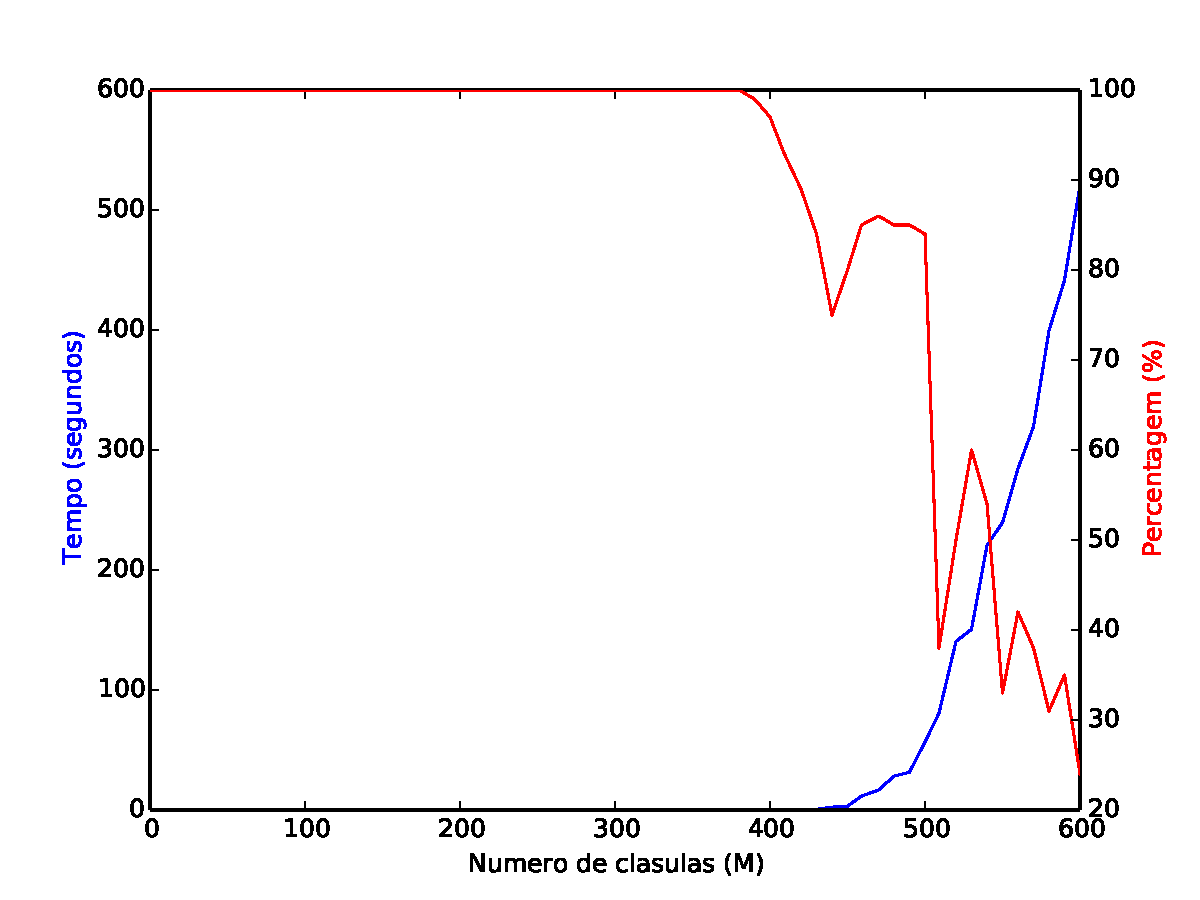
\includegraphics[height=10cm]{images/max3sat_100at}
			\caption{Curva de resposta de tempo (azul), curva de percentagem (vermelho)}
			\label{fig:max3sat100at}
		\end{figure}
		
 \subsection{Experimento 2}
	\subsubsection{Descrição}
		Para $K = 2$ (ou seja, 2-SAT) e $N = 100$, levantar a curva de resposta de tempo, e apresentá-la sobreposta à curva de percentagem de problemas satisfazíveis. Cada ponto deve ser obtido a partir de pelo menos 100 instâncias geradas aleatoriamente. Apresentar e discutir o formato do gráfico.
	\subsubsection{Resultados}
		Da mesma forma que o gráfico em ~\ref{subsec:resultadosExp1}, a figura ~\ref{fig:max2sat100at} mostra os tempos promedio de resposta e o percentagem de instâncias satisfazíveis, mas esta vez tem as instâncias são $K$-literais com $K=2$. Neste caso o percentagem de instâncias satisfazíveis diminui rápidamente ainda para valores $M/N$ muito próximo de 1. Por outro lado, no gráfico mostra que para valores entre 200 e 300 cláusulas o tempo promedio de resposta é consideravelmente mais grande que para outros valores em que seu tempo é muito próximo a 0.
		\begin{figure}[H]
			\centering
			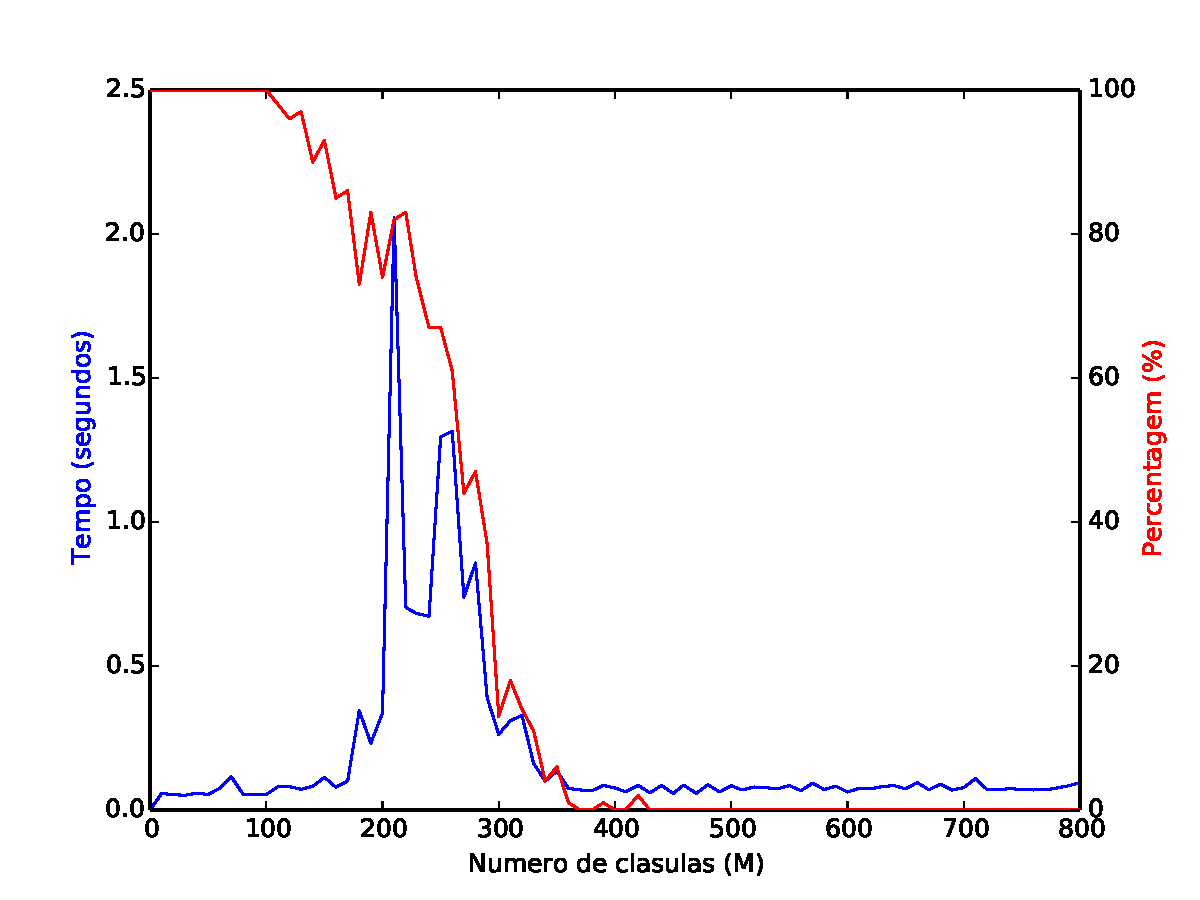
\includegraphics[height=10cm]{images/max2sat_100at}
			\caption{Curva de resposta de tempo (azul), curva de percentagem (vermelho)}
			\label{fig:max2sat100at}
		\end{figure}
		
		
\subsection{Experimento 3}
	\subsubsection{Descrição}
		Apresentar 5 gráficos mostrando o tempo de execução em função de $N$ para $K = 3$. Em cada gráfico, o valor de $M / N$ deve ser fixo. Os cinco gráficos devem ser feitos para $N$ variando de 100 a 1000, em intervalos de 100. Os valores de $M / N$ de cada um dos 5 gráficos são 1; 3; 4,3; 6; e 8. Discutir a natureza da curva obtida em cada caso, se polinomial ou exponencial. 
	\subsubsection{Resultados}
		Na tabela~\ref{tab:3satTempos} mostra os tempos promedio em segundos de cada configuração de parâmetros. Para as relações $M/N=1.0$ e $M/N=3.0$ os tempos são menores a 1 segundo, mas para $M/N=4.3$ os tempos são consideravelmente mais grandes levando pouco mais de uma hora para $N=1000$. Além, para $M/N=6.0$ os tempos são muito grandes levando mais de um dia para seu execução com $N=600$ e sem calcular para valores de $N$ maiores. Porém, para $M/N=8.0$ os tempos não aumentam muito apesar de ter muitas cláusulas, e como se mostrou em ~\ref{subsec:resultadosExp1} não tem muitas instâncias satisfazíveis, portanto pode conclui-se que esta relação não é muito dependente de $N$ porque na maioria das vezes as instâncias são insatisfazíveis.
		\begin{table}[H]
			\centering{
				\resizebox{.9\columnwidth}{!}{
					\begin{tabular}{|c|r|r|r|r|r|} \hline
						\multicolumn{1}{|c|}{{N}} & \multicolumn{1}{|c|}{{$M/N=1.0$}} & \multicolumn{1}{|c|}{{$M/N=3.0$}} & \multicolumn{1}{|c|}{{$M/N=4.3$}} & \multicolumn{1}{|c|}{{$M/N=6.0$}} & \multicolumn{1}{|c|}{{$M/N=8.0$}} \\ \cline{1-6}
						100    & 0.042 & 0.050 & 10.278  & 6327.574 & 100.724 \\\hline
						200    & 0.092 & 0.137 & 58.735  & 7732.361 & 224.791 \\\hline
						300    & 0.071 & 0.108 & 116.031 & 15253.935 & 384.112 \\\hline
						400    & 0.131 & 0.322 & 230.58 & 40823.234 & 681.084 \\\hline
						500    & 0.178 & 0.434 & 512.05 & 91834.454 & 800.268 \\\hline
						600    & 0.196 & 0.422 & 741.912 & 131082.805 & 811.481 \\\hline
						700    & 0.168 & 0.668 & 998.048 & - & 811.101 \\\hline
						800    & 0.188 & 0.763 & 1806.502 & -  & 842.849 \\\hline
						900    & 0.296 & 0.765 & 2501.011 & -  & 895.298 \\\hline
						1000  & 0.199 & 0.717 & 4700.17 & - & 874.026 \\\hline
					\end{tabular}
        				}
			}
			\caption{Comparação de tempos (segundos) de Max 3-SAT}									\label{tab:3satTempos}
		\end{table}

		A figura~\ref{fig:max3satmn10} mostra os tempos para $M/N=1.0$. Esta curva tem um comportamento polinomial, quase lineal, porque os tempos aumentan proporcionalmente a $N$ ainda para $N=1000$.
		\begin{figure}[H]
			\centering
			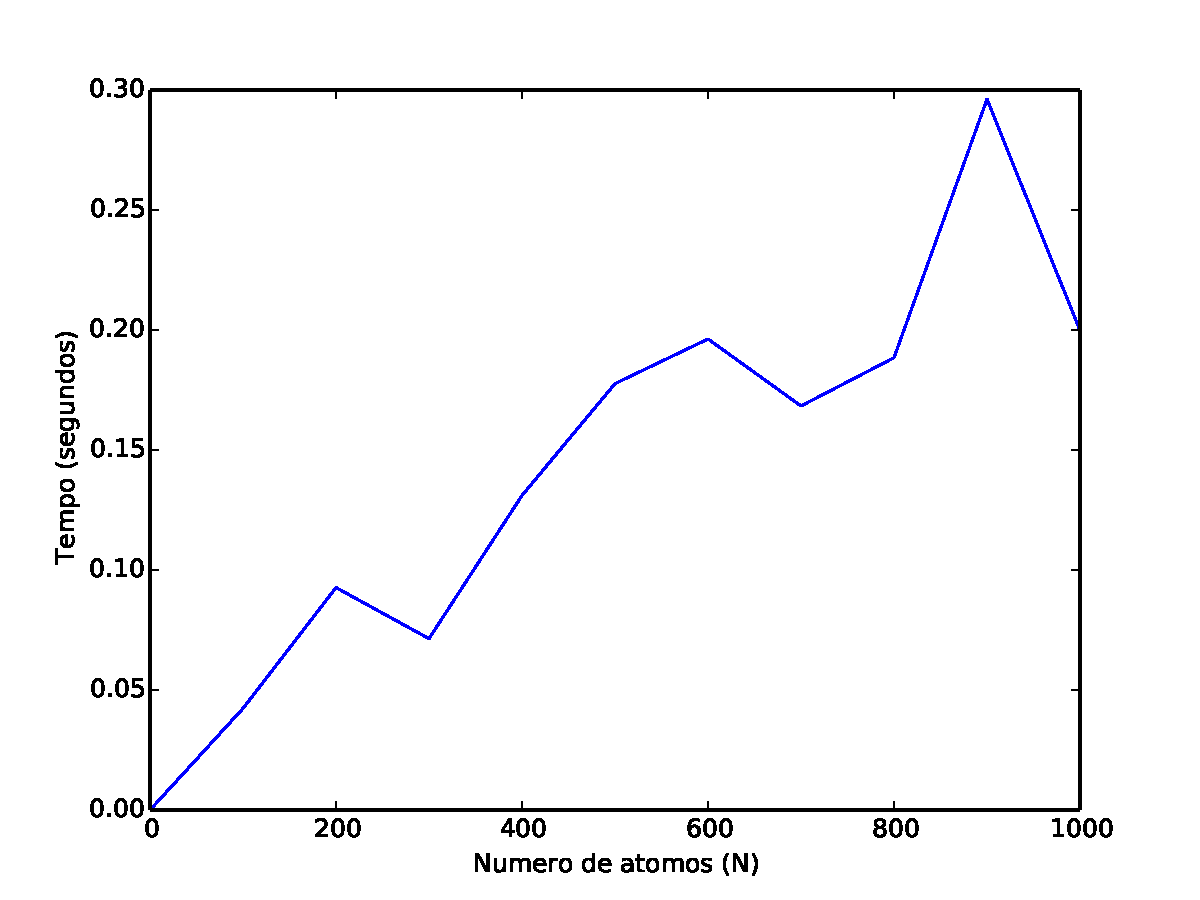
\includegraphics[height=8cm]{images/max3sat_mn10}
			\caption{Curva de resposta de tempo para $M/N=1.0$}
			\label{fig:max3satmn10}
		\end{figure}
		
		Da mesma forma que a figura anterior, a figura~\ref{fig:max3satmn30} mostra uma curva com comportamento polinomial, mas com tempos maiores.
		\begin{figure}[H]
			\centering
			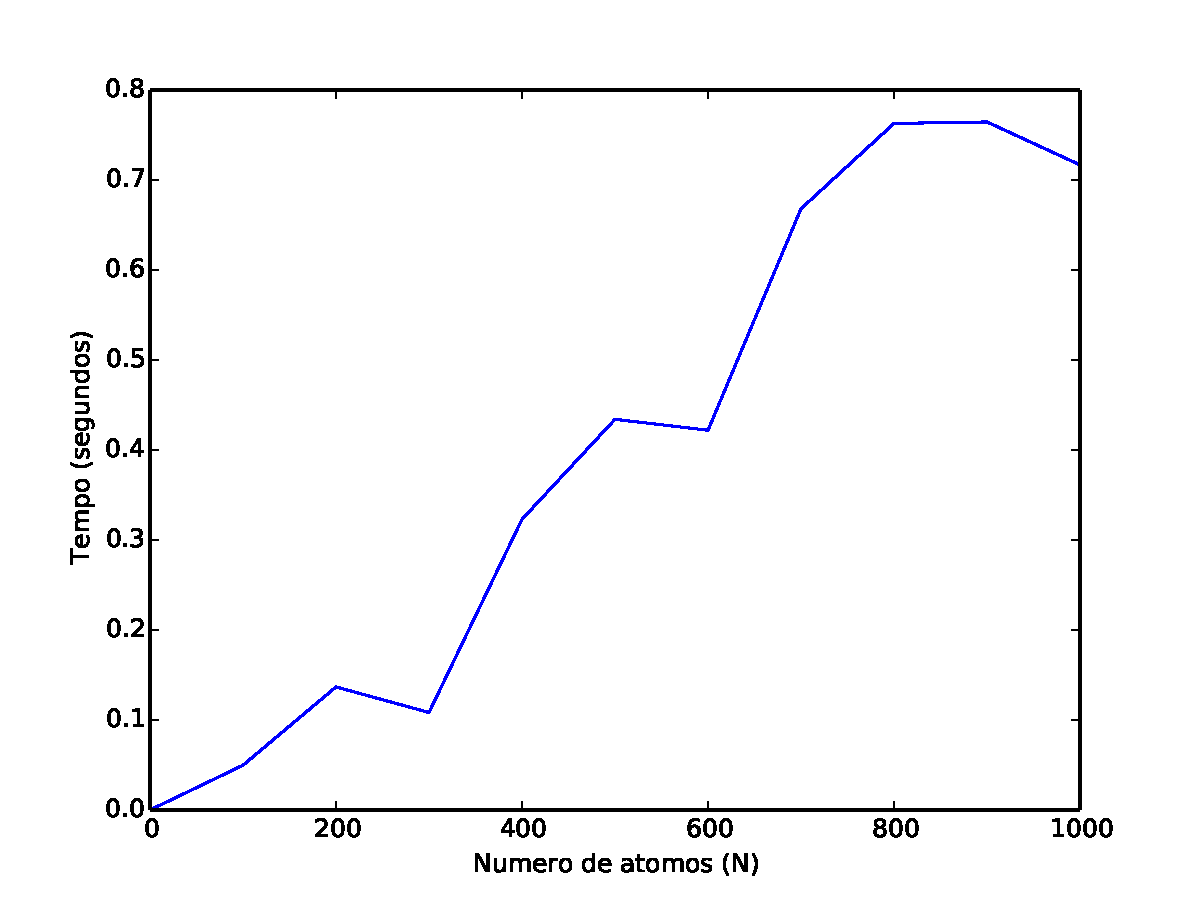
\includegraphics[height=8cm]{images/max3sat_mn30}
			\caption{Curva de resposta de tempo para $M/N=3.0$}
			\label{fig:max3satmn30}
		\end{figure}
		
		Para $M/N=4.3$ a curva de resposta de tempo tem um comportamento exponencial como mostra a figura~\ref{fig:max3satmn43} com tempos muito grandes de mais de uma hora (para $N=1000$). Os aumentos de tempo são maiores enquanto o valor $N$ continúa aumentando.
		\begin{figure}[H]
			\centering
			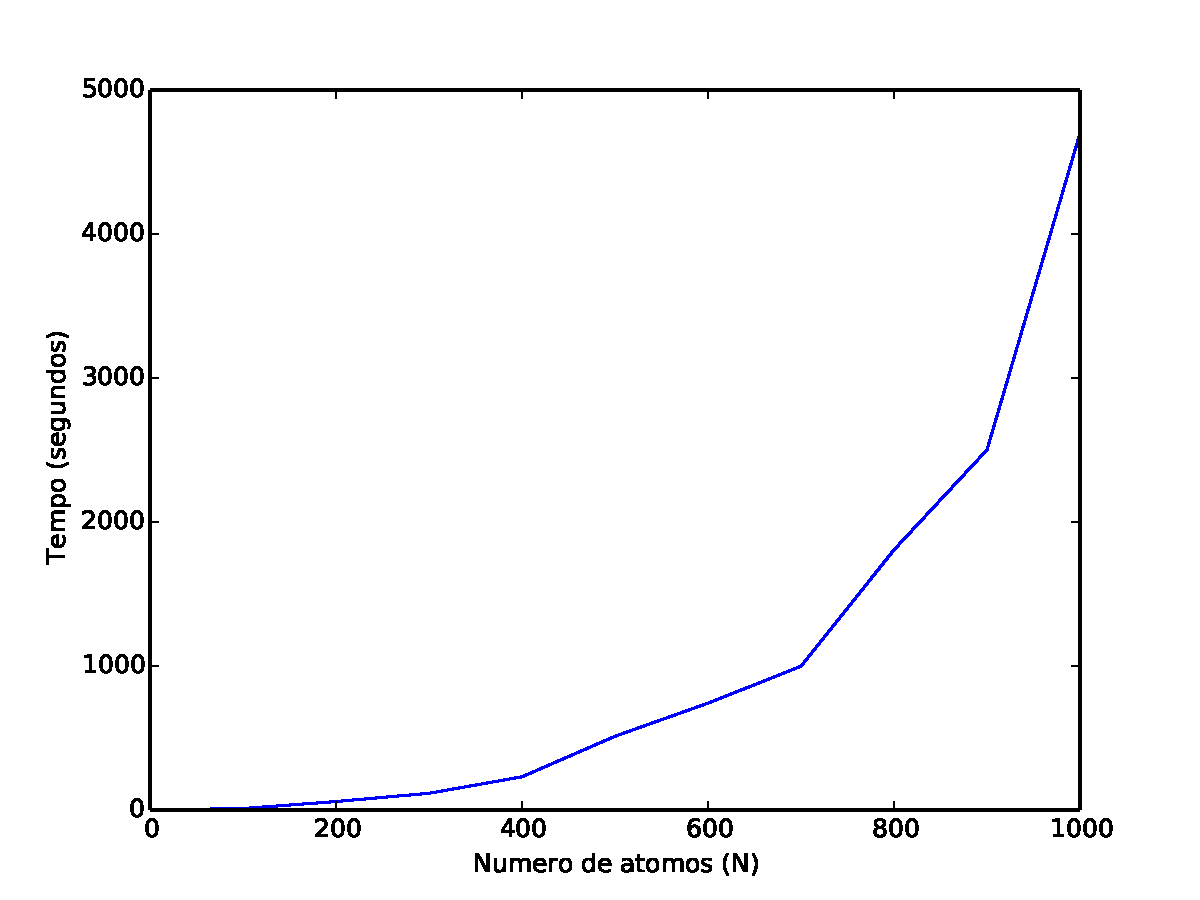
\includegraphics[height=8cm]{images/max3sat_mn43}
			\caption{Curva de resposta de tempo para $M/N=4.3$}
			\label{fig:max3satmn43}
		\end{figure}
		
		Tão como mostrava a figura~\ref{fig:max3satmn43}, na curva mostrada na figura~\ref{fig:max3satmn60} tem um comportamento exponencial com tempos de mais de um dia para $N=600$.
		\begin{figure}[H]
			\centering
			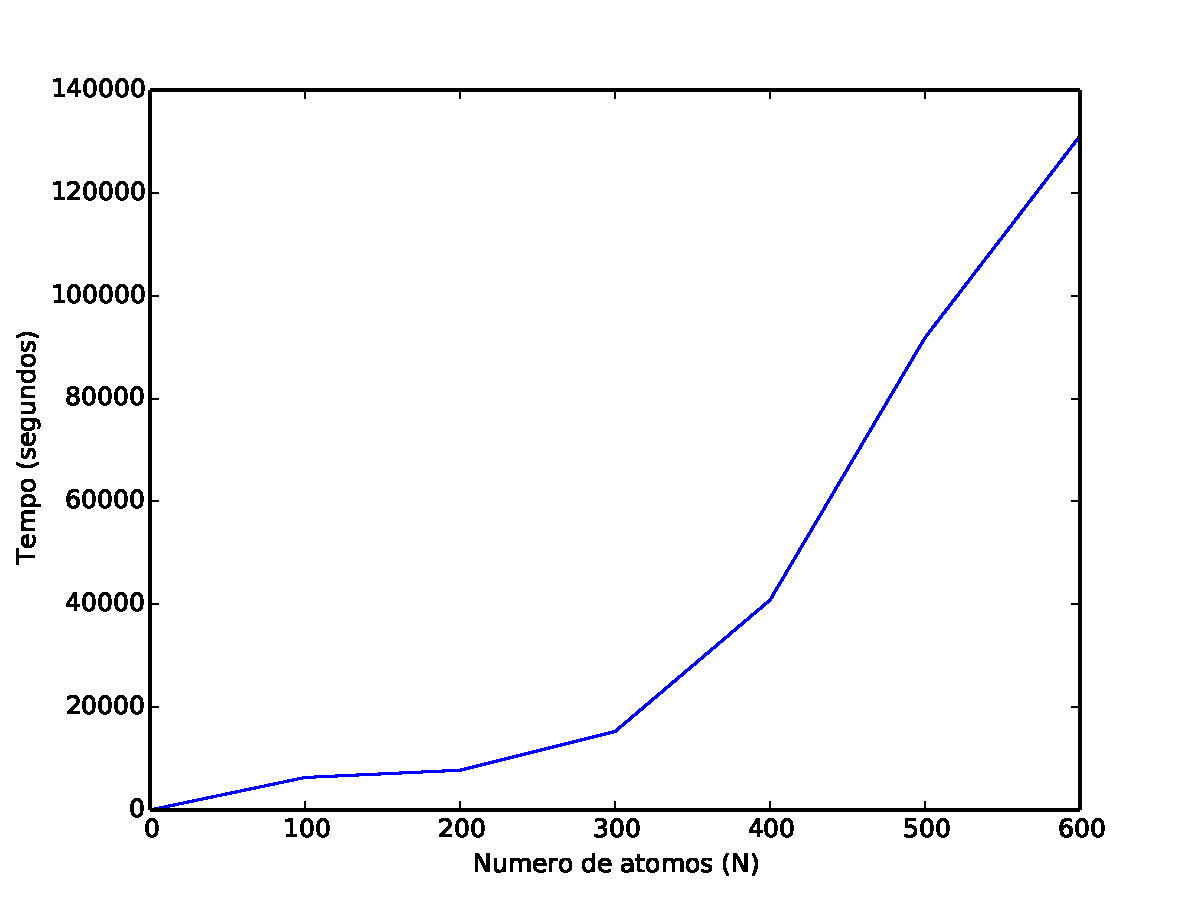
\includegraphics[height=8cm]{images/max3sat_mn60}
			\caption{Curva de resposta de tempo para $M/N=6.0$}
			\label{fig:max3satmn60}
		\end{figure}
		
		Por último, a figura~\ref{fig:max3satmn80} mostra novamente uma curva de comportamento polinomial que já foi explicado ao inicio desta seção.
		\begin{figure}[H]
			\centering
			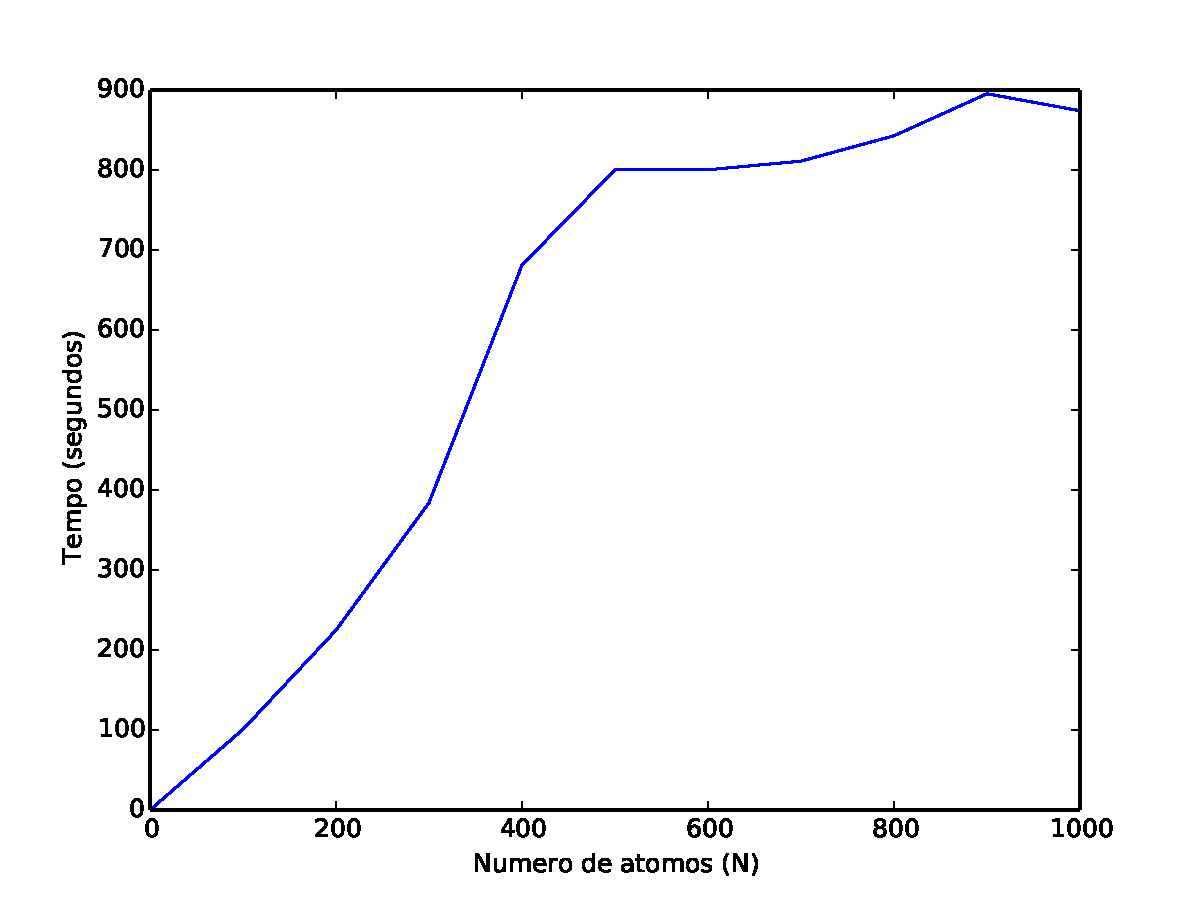
\includegraphics[height=8cm]{images/max3sat_mn80}
			\caption{Curva de resposta de tempo para $M/N=8.0$}
			\label{fig:max3satmn80}
		\end{figure}

\subsection{Experimento 4}
	\subsubsection{Descrição}
		Apresentar 5 gráficos mostrando o tempo de execução em função de $N$ para $K = 2$. Em cada gráfico, o valor de $M / N$ deve ser fixo. Os cinco gráficos devem ser feitos para $N$ variando de 100 a 1000, em intervalos de 100. Os valores de $M / N$ de cada um dos 5 gráficos são 1; 3; 4,3; 6; e 8. Discutir a natureza da curva obtida em cada caso, se polinomial ou exponencial.
	
	\subsubsection{Resultados}
		Na tabela~\ref{tab:2satTempos} tem a mesma informação que a tabela~\ref{tab:3satTempos} mas para instâncias com $K=2$. Em geral, enquanto a relação $M/N$ aumenta os tempos vão aumentando também. Em $M/N=3.0$ os tempos são menores a 1 segundo, excepto para $N=200$ que pode deve-se a instâncias muito complicadas para o programa, esto é possível porque a geração de dados é totalmente aleatória. Além, pode-se notar que as diferencias entre os tempos para as diferentes relações não são muito diferente numa de outra, sendo apenas 2 segundos para $M/N=8.0$ e $N=1000$.
		\begin{table}[H]
			\centering{
				\resizebox{.9\columnwidth}{!}{
					\begin{tabular}{|c|r|r|r|r|r|} \hline
						\multicolumn{1}{|c|}{{N}} & \multicolumn{1}{|c|}{{$M/N=1.0$}} & \multicolumn{1}{|c|}{{$M/N=3.0$}} & \multicolumn{1}{|c|}{{$M/N=4.3$}} & \multicolumn{1}{|c|}{{$M/N=6.0$}} & \multicolumn{1}{|c|}{{$M/N=8.0$}} \\ \cline{1-6}
						100    & 0.040 & 0.259 & 0.057  & 0.063 & 0.075 \\\hline
						200    & 0.048 & 18.241 & 0.078  & 0.099 & 0.136 \\\hline
						300    & 0.052 & 0.076 & 0.111 & 0.152 & 0.218 \\\hline
						400    & 0.062 & 0.128 & 0.159 & 0.221 & 0.354 \\\hline
						500    & 0.060 & 0.115 & 0.193 & 0.337 & 0.615 \\\hline
						600    & 0.076 & 0.188 & 0.310 & 0.446 & 0.700 \\\hline
						700    & 0.073 & 0.191 & 0.382 & 0.659 & 0.982 \\\hline
						800    & 0.073 & 0.217 & 0.398 & 0.890  & 1.184 \\\hline
						900    & 0.0790 & 0.272 & 0.551 & 1.128 & 2.731 \\\hline
						1000  & 0.286 & 0.359 & 0.582 & 1.535 & 2.275 \\\hline
					\end{tabular}
        				}
			}
			\caption{Comparação de tempos (segundos) de Max 2-SAT}
			\label{tab:2satTempos}
		\end{table}
		
		A figura~\ref{fig:max2satmn10} mostra os tempos para $M/N=1.0$. Esta curva tem um comportamento polinomial e com aumentos de tempo proporcionais a $N$.
		\begin{figure}[H]
			\centering
			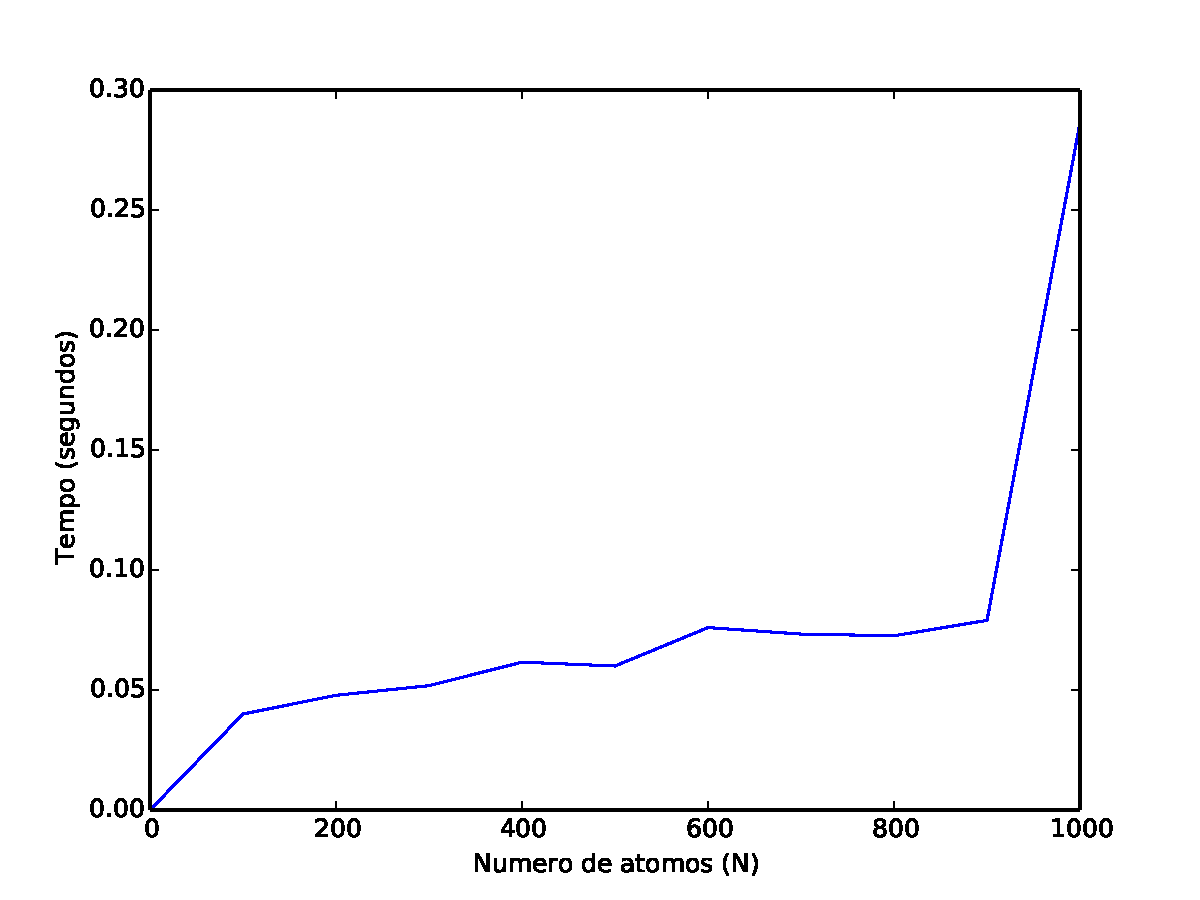
\includegraphics[height=8cm]{images/max2sat_mn10}
			\caption{Curva de resposta de tempo para $M/N=1.0$}
			\label{fig:max2satmn10}
		\end{figure}
		
		Em geral a figura a figura~\ref{fig:max2satmn30} mostra uma curva de comportamento polinomial, mas com uma anormalidade em $N=200$ que já foi explicado anteriormente.
		\begin{figure}[H]
			\centering
			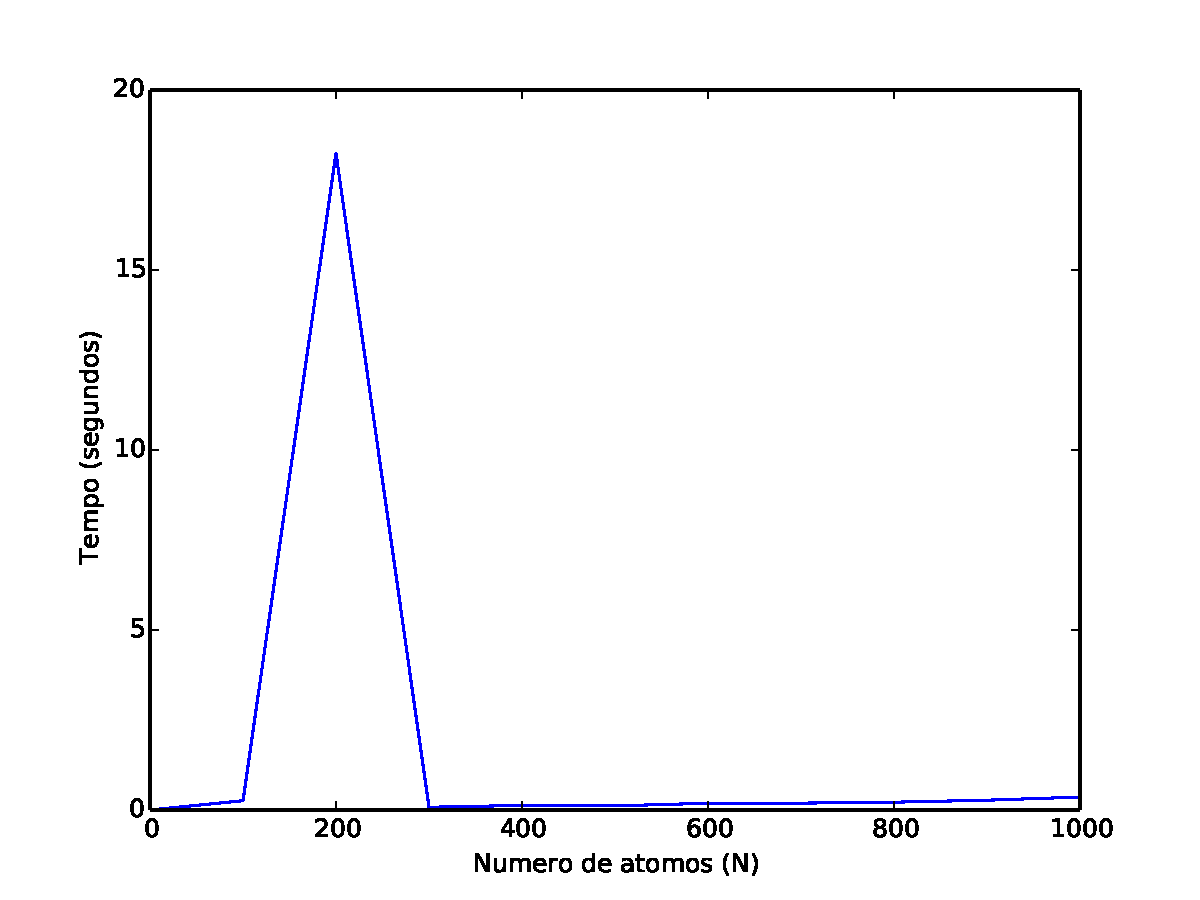
\includegraphics[height=8cm]{images/max2sat_mn30}
			\caption{Curva de resposta de tempo para $M/N=3.0$}
			\label{fig:max2satmn30}
		\end{figure}
		
		Para $M/N=4.3$ a curva mostrada na figura~\ref{fig:max2satmn43} tem um comportamento polinomial, além já começa a ser quase lineal em $N$ a diferencia das figuras anteriores.
		\begin{figure}[H]
			\centering
			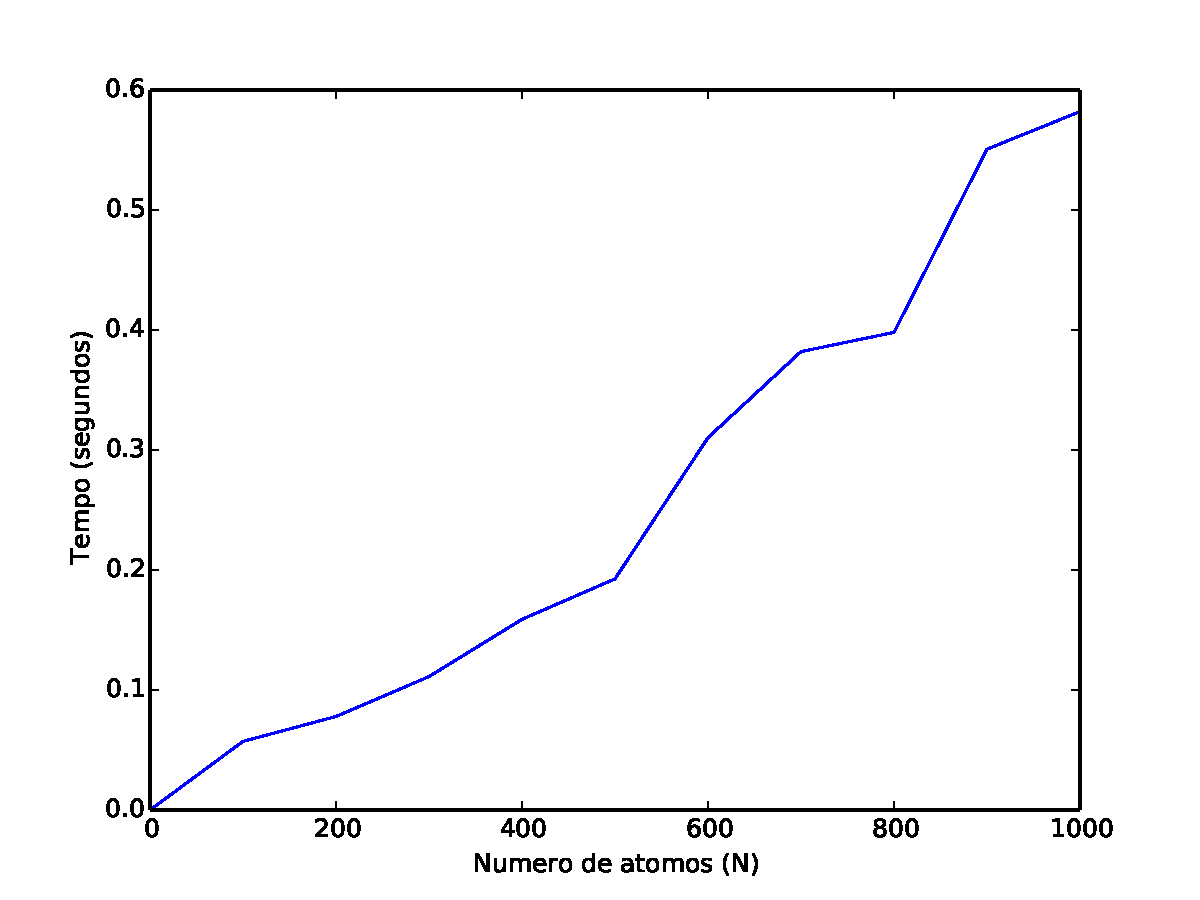
\includegraphics[height=8cm]{images/max2sat_mn43}
			\caption{Curva de resposta de tempo para $M/N=4.3$}
			\label{fig:max2satmn43}
		\end{figure}
		
		A figura~\ref{fig:max2satmn60} já tem uma curva de comportamento exponencial depois de que a figura anterior mostra-se que a curva já estava sendo quase lineal.
		\begin{figure}[H]
			\centering
			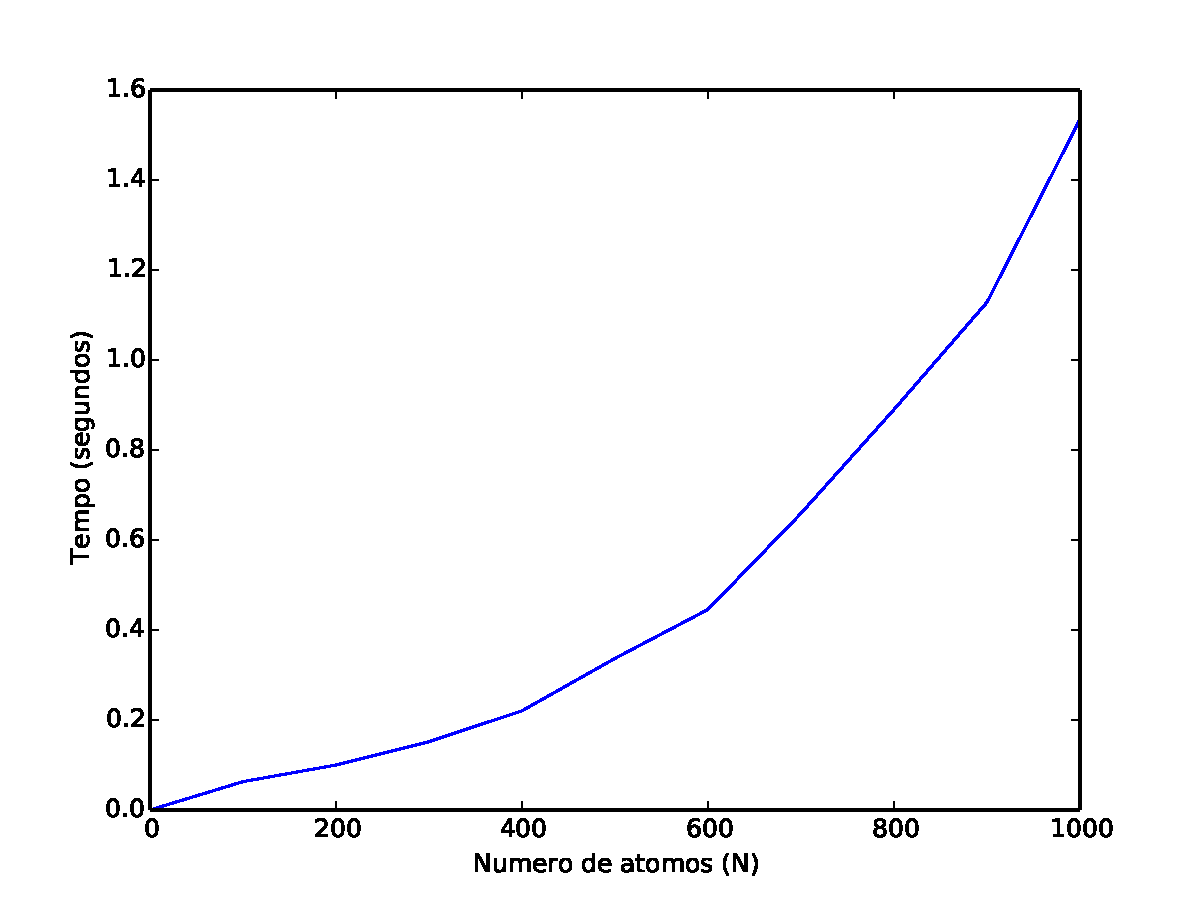
\includegraphics[height=8cm]{images/max2sat_mn60}
			\caption{Curva de resposta de tempo para $M/N=6.0$}
			\label{fig:max2satmn60}
		\end{figure}
		
		Por último, a figura~\ref{fig:max2satmn80} continúa mostrando uma curva exponencial para $M/N=8.0$.
		\begin{figure}[H]
			\centering
			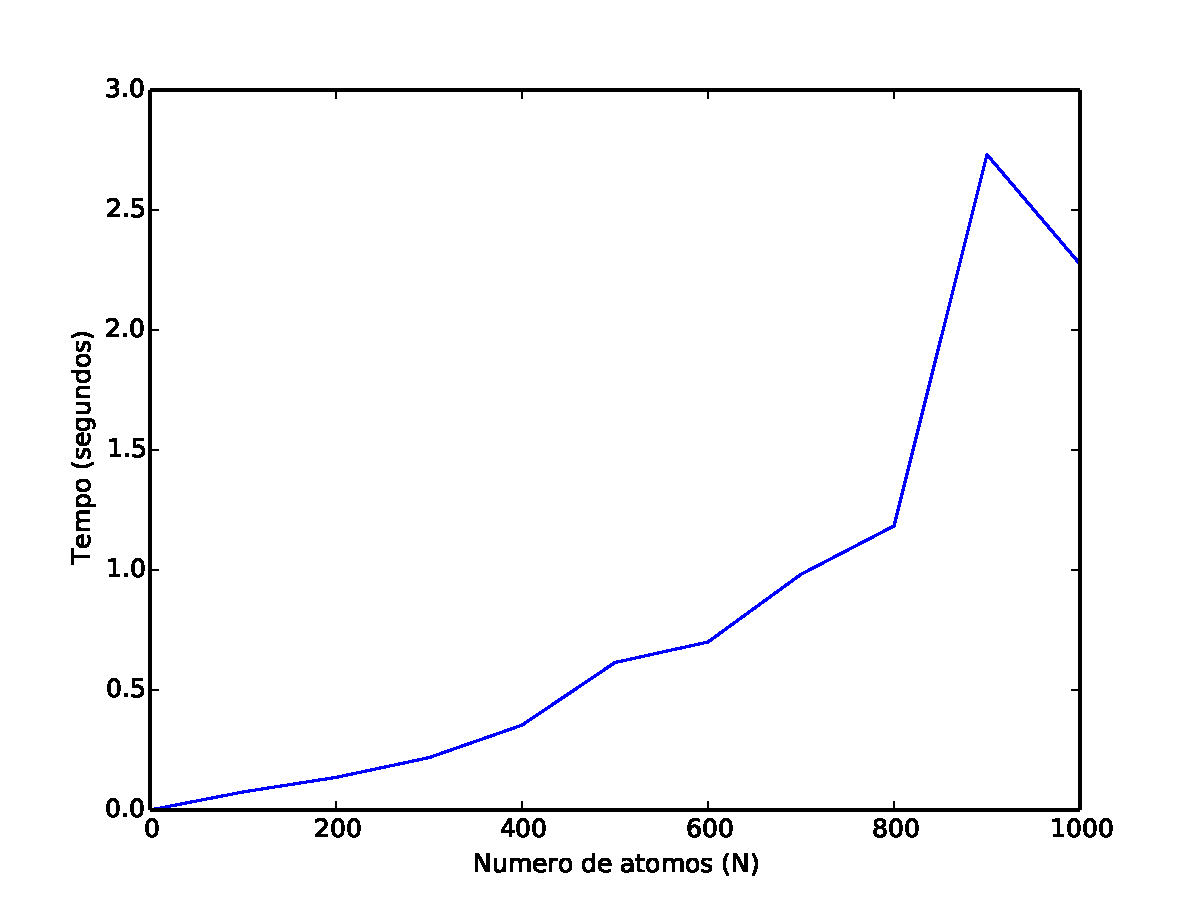
\includegraphics[height=8cm]{images/max2sat_mn80}
			\caption{Curva de resposta de tempo para $M/N=8.0$}
			\label{fig:max2satmn80}
		\end{figure}